\documentclass[10pt, compress]{beamer}

\usetheme{m}
\usepackage{subfigure}
\usepackage{caption}
\usepackage{color}
\usepackage{tikz}
\usepackage{float}
\usepackage{pgfplots}
\usepackage[spanish,es-tabla,es-noquoting,activeacute]{babel}
\setcounter{tocdepth}{3}
\decimalpoint

\pgfplotscreateplotcyclelist{cuatro}{%
{mark=*, color=red, mark size=3},
{mark=triangle*, color=blue, mark size=3},
{mark=square*, color=brown, mark size=4},
{mark=x, color=black, mark size=4}
}

\usetikzlibrary{backgrounds,arrows,positioning,automata,shadows}
\usepackage[font={large,bf}]{caption}

\newcommand{\graphic}[1]{
    \resizebox{0.45\textwidth}{0.35\textheight}{
        \input{graficos/#1}
    }
}

\usepackage{multicol}
\usepackage[backend=bibtex,sorting=ynt]{biblatex}

\addbibresource{bib}

\newcommand{\shortt}{Cuando los chicos son mejores}


\title{Cuando los chicos son mejores}
\subtitle{When children are better (or at least more open-minded) learners than adults: Developmental differences in learning the forms of causal relationships}

\author{Escrito por: Lucas, et al., aceptado en Diciembre 2013 \\(Universidades: Edinburhgh y Berkeley)}

\institute{
\begin{center}
Presentado por: Luciano Gandini y Pablo Brusco\\
 Departamento de Computación, FCEN, UBA \\
\vspace{0.2cm}
\end{center}
}

\begin{document}

\maketitle


% \begin{frame}
% \frametitle{Contenidos}
% \tableofcontents
% \end{frame}

\section{Experimento}


\begin{frame}[fragile]{\shortt: Experimento, Quilombo}

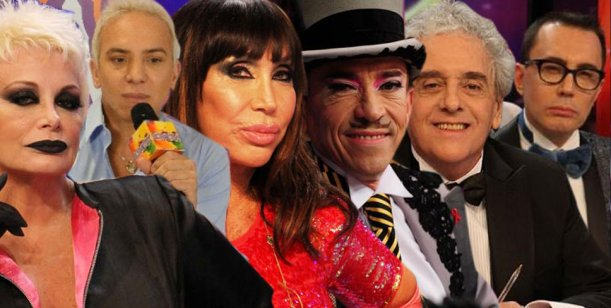
\includegraphics[width=0.7\textwidth]{images/quilombo.jpg}
\bigskip

Empecemos con un experimento

\end{frame}


\section{Grupo 1}
\begin{frame}[fragile]{\shortt: Experimento, Quilombo}
\begin{center}
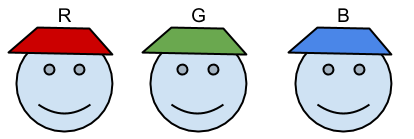
\includegraphics[scale=0.3]{images/caras1.png}
\end{center}
\bigskip

\only<1>{
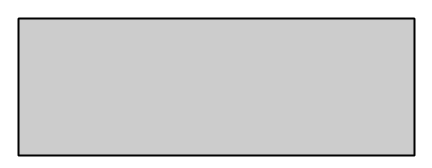
\includegraphics[scale=0.3]{images/fondo1.png}
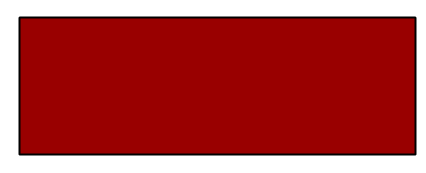
\includegraphics[scale=0.3]{images/fondo2.png}
}

\only<2>{
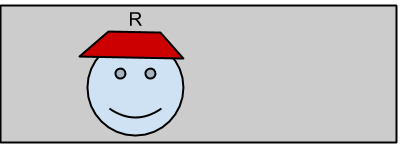
\includegraphics[scale=0.3]{images/e1.png}
}

\only<3>{
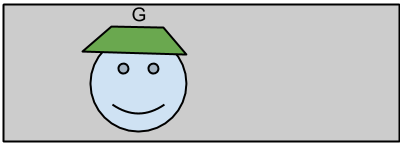
\includegraphics[scale=0.3]{images/e2.png}
}

\only<4>{
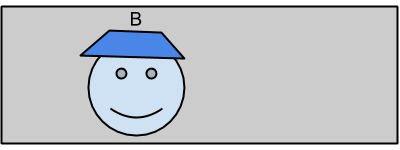
\includegraphics[scale=0.3]{images/e3.png}
}

\only<5>{
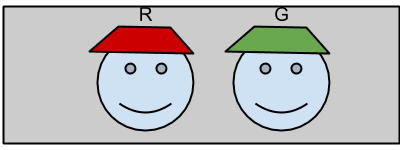
\includegraphics[scale=0.3]{images/e4.png}
}

\only<6>{
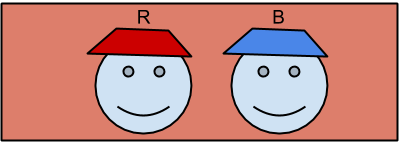
\includegraphics[scale=0.3]{images/e5.png}
}

\only<7>{
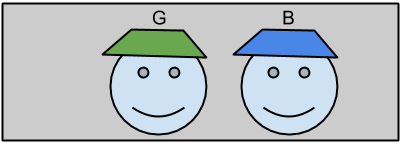
\includegraphics[scale=0.3]{images/e6.png}
}

\only<8>{
\begin{center}
    Para escribir en su hoja: Cuál de los sujetos consideran quilomberos?
\end{center}
}


\end{frame}
\begin{frame}[fragile]{\shortt: Experimento, Quilombo}
\begin{center}
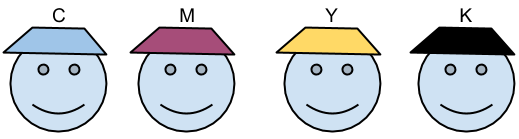
\includegraphics[scale=0.3]{images/caras2.png}
\end{center}
\bigskip

\only<2>{
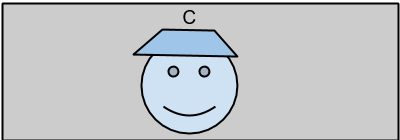
\includegraphics[scale=0.3]{images/t1.png}
}

\only<3>{
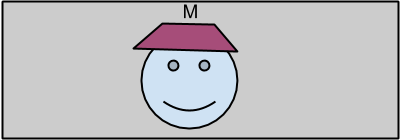
\includegraphics[scale=0.3]{images/t2.png}
}

\only<4>{
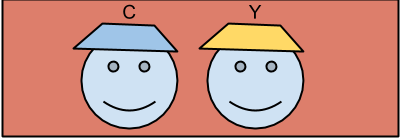
\includegraphics[scale=0.3]{images/t3.png}
}

\only<5>{
\begin{center}
    Para escribir en su hoja: Cuál de los sujetos consideran quilomberos?
\end{center}
}


\end{frame}


\section{Grupo 2}
\begin{frame}[fragile]{\shortt: Experimento, Quilombo}
\begin{center}
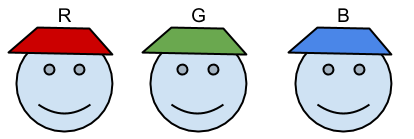
\includegraphics[scale=0.3]{images/caras1.png}
\end{center}
\bigskip

\only<1>{
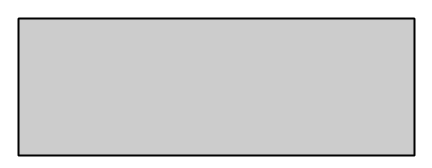
\includegraphics[scale=0.3]{images/fondo1.png}
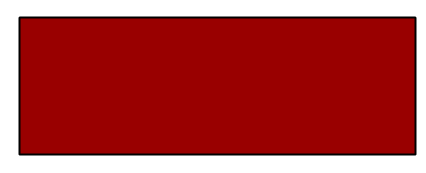
\includegraphics[scale=0.3]{images/fondo2.png}
}

\only<2>{
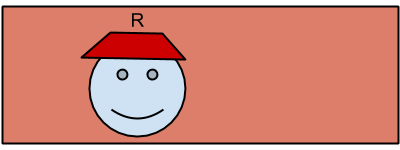
\includegraphics[scale=0.3]{images/h1.png}
}

\only<3>{
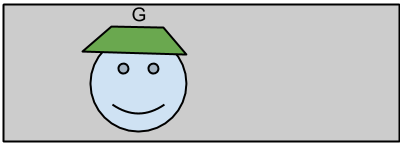
\includegraphics[scale=0.3]{images/h2.png}
}

\only<4>{
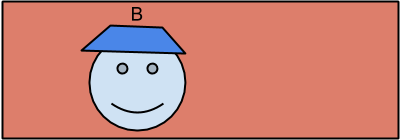
\includegraphics[scale=0.3]{images/h3.png}
}

\only<5>{
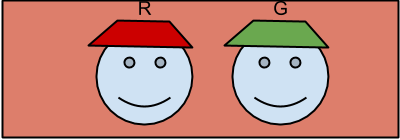
\includegraphics[scale=0.3]{images/h4.png}
}

\only<6>{
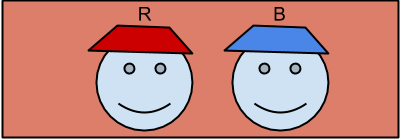
\includegraphics[scale=0.3]{images/h5.png}
}

\only<7>{
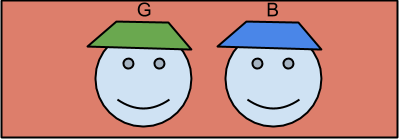
\includegraphics[scale=0.3]{images/h6.png}
}

\only<8>{
\begin{center}
    Para escribir en su hoja: Cuál de los sujetos consideran quilomberos?
\end{center}
}


\end{frame}
\begin{frame}[fragile]{\shortt: Experimento, Quilombo}
\begin{center}
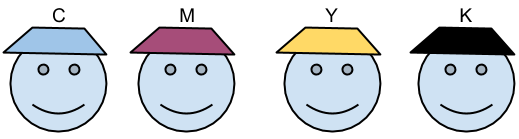
\includegraphics[scale=0.3]{images/caras2.png}
\end{center}
\bigskip

\only<2>{
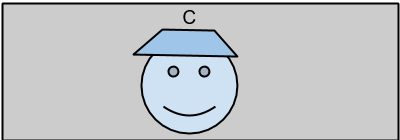
\includegraphics[scale=0.3]{images/t1.png}
}

\only<3>{
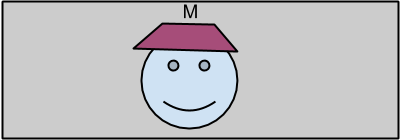
\includegraphics[scale=0.3]{images/t2.png}
}

\only<4>{
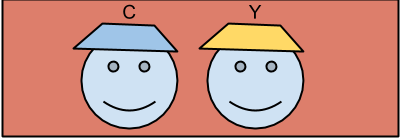
\includegraphics[scale=0.3]{images/t3.png}
}

\only<5>{
\begin{center}
    Para escribir en su hoja: Cuál de los sujetos consideran quilomberos?
\end{center}
}


\end{frame}



\section{Introducción}


\begin{frame}[fragile]{\shortt: Hipótesis}

\begin{center}
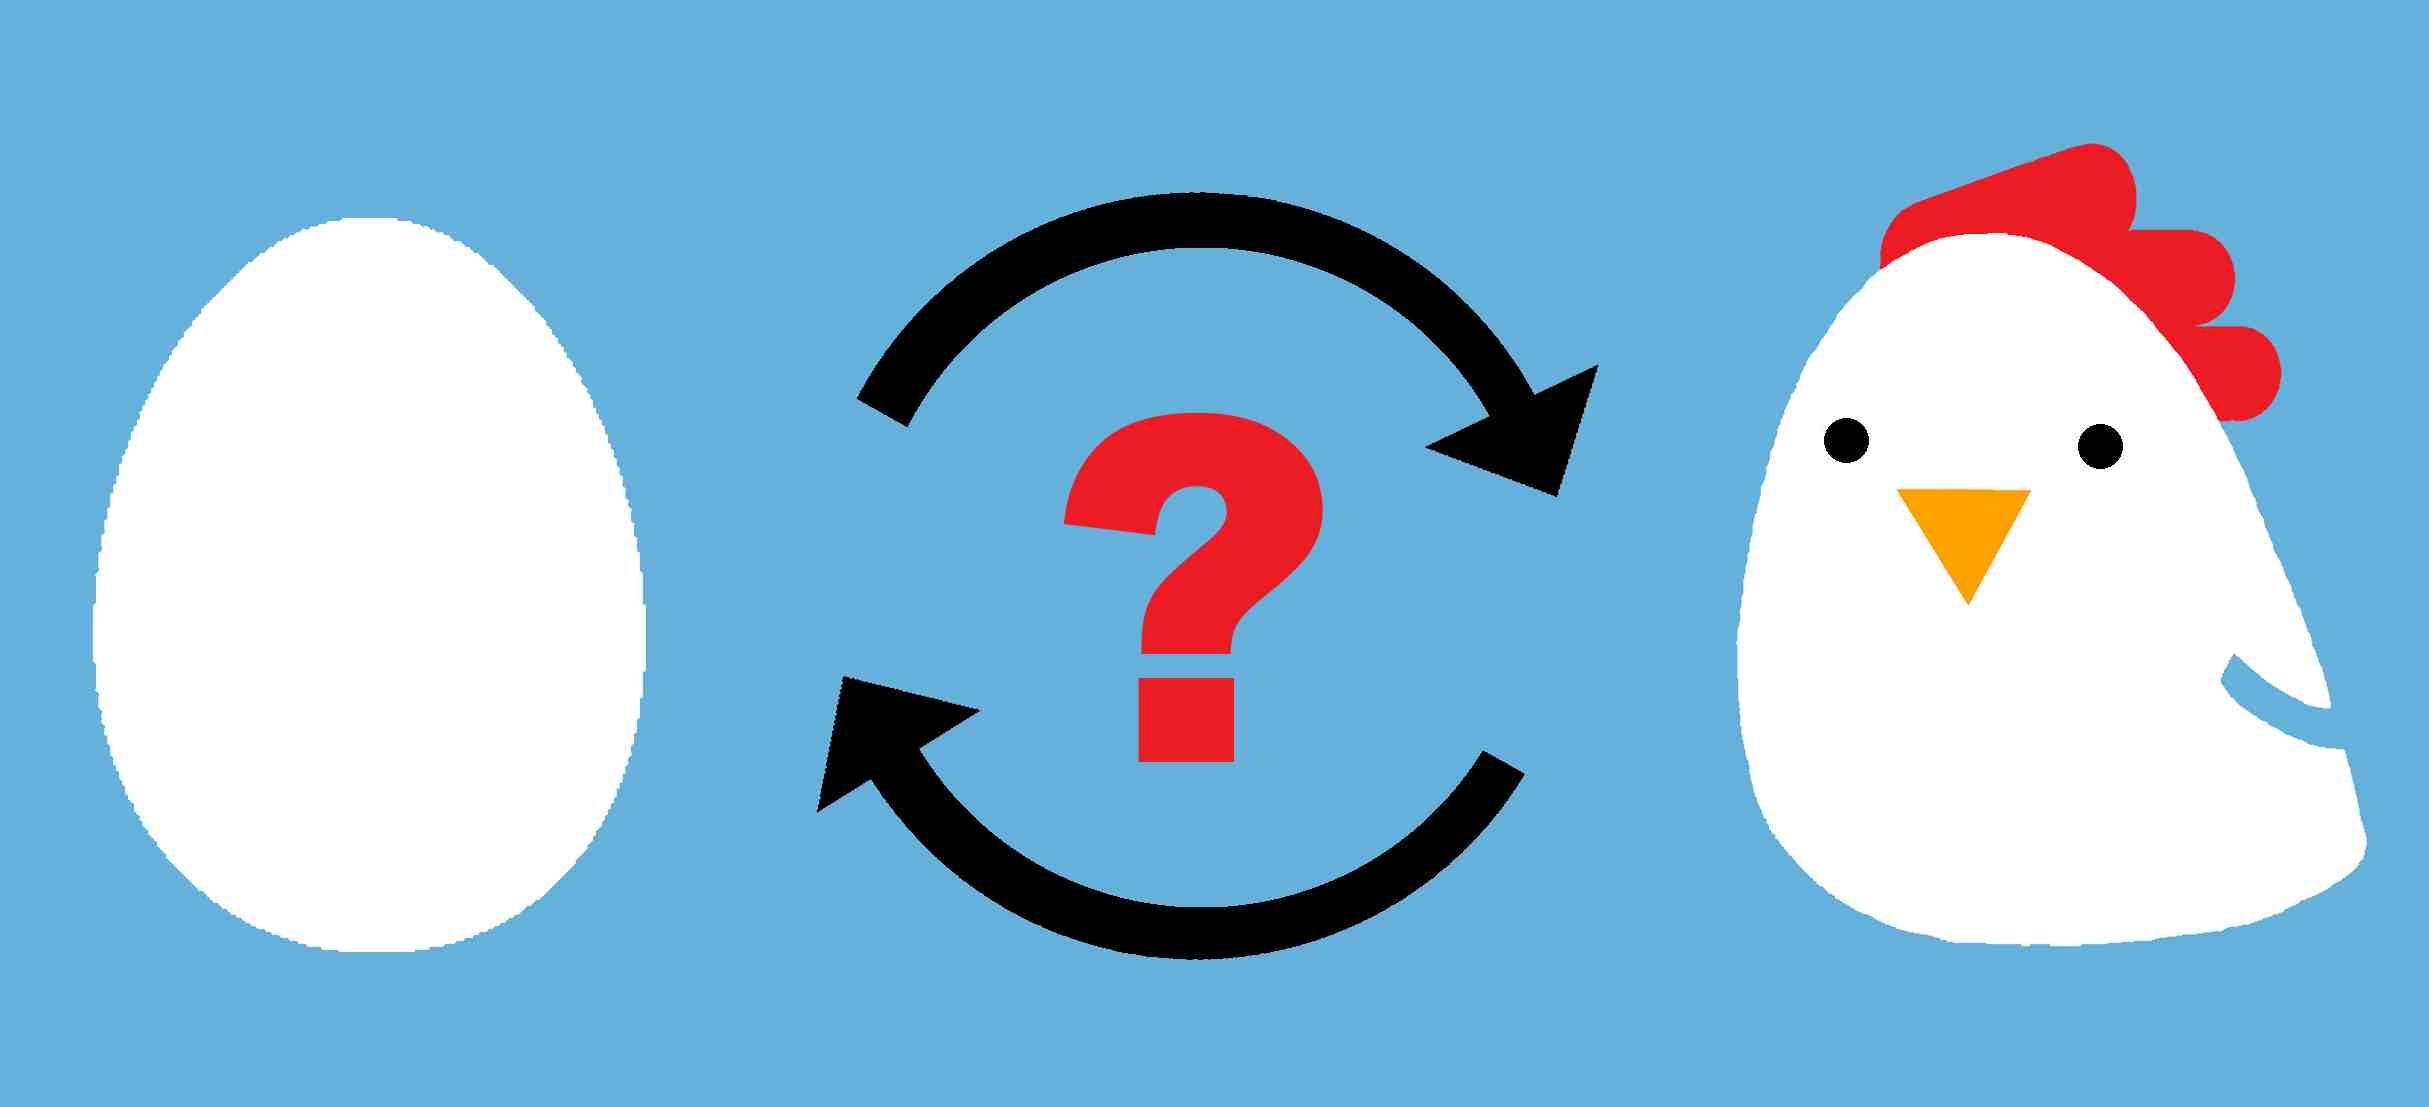
\includegraphics[scale=0.05]{images/gallina.jpg}
\end{center}
\begin{block}{Hipótesis}
\begin{itemize}
\item Los niños aprenden \alert{relaciones causales} velozmente y realizan inferencia causal de gran alcance a partir de observaciones. 

\item Los adultos pueden aprender estas relaciones, pero la experiencia hace que sus conclusiones estén sesgadas. 

\end{itemize}
\end{block}
\end{frame}

\begin{frame}[fragile]{\shortt: Trabajo Previo}


\begin{block}{Hasta el momento de publicación}

\begin{itemize}
\item No había estudios mostrando que los niños pueden aprender principios abstractos sobre la forma lógica de relaciones causales.
\item En consecuencia, tampoco comparaciones entre niños y adultos en su habilidad para realizarlo.
\item En el trabajo de \alert{Lucas and Griffiths (2010)} se encontró que los adultos pueden aprender \alert{sobrehipótesis} sobre relaciones causales y explicarlas en términos de un modelo Bayesiano jerárquico. Además, muestra que los adultos suelen estar predispuestos a relaciones disyuntivas y aprenden estas relaciones con mayor facilidad que las conjuntivas.
\end{itemize}    



\end{block}

\end{frame}

\begin{frame}[fragile]
\begin{block}{Sobre-hipótesis}
Se probaron dos principios causales:
\begin{itemize}
\item Forma disyuntiva: cada causa tiene una probabilidad independiente de causar un efecto.
\item Forma conjuntiva: causas independientes no pueden producir un efecto, pero el conjunto de ellas si.
\end{itemize}
\end{block}

\pause
Pero.. ¿Cuán buenos son los niños aprendiendo las sobrehipótesis?

\begin{exampleblock}{Pregunta}
¿Intuitivamente debería costarles más o menos que a los adultos? 
\end{exampleblock}

\pause
Varias investigaciones con enfoque Bayesiano indican que los niños tienen priors más débiles que le permiten adoptar nuevas hipótesis fácilmente y sin sesgos.


\end{frame}

\section{Metodología}

\begin{frame}[fragile]
  \frametitle{\shortt:  Experimento 1}
    \begin{block}{Problemas de comunicación}
        Los niños suelen tener dificultades articulando hipótesis causales explícitamente, por lo que se diseño un experimento que sólo requiere criterios positivos/negativos.
    \end{block}
    \begin{center}
    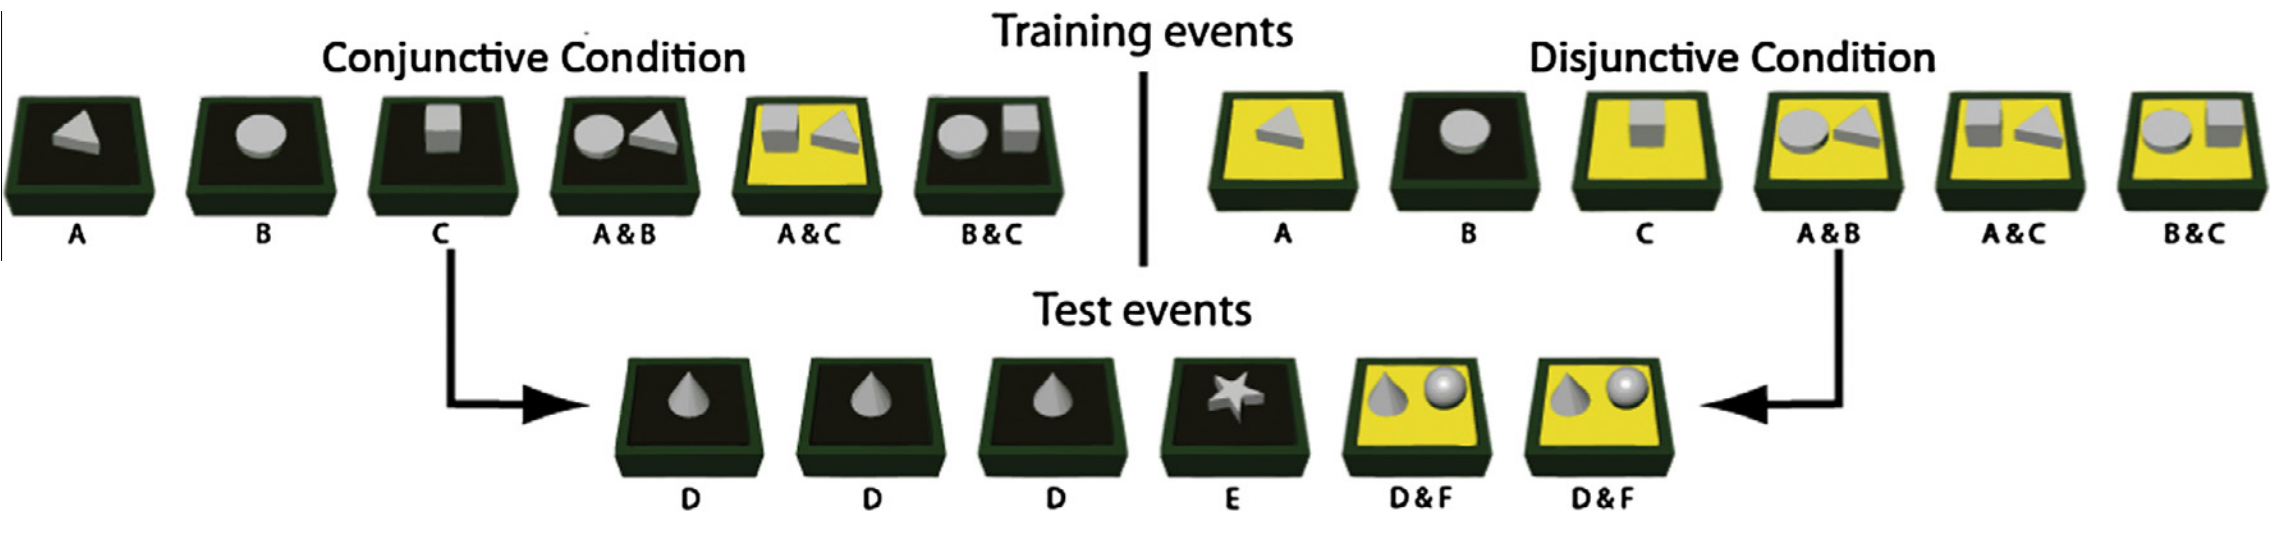
\includegraphics[scale=0.25]{images/experiment1.png}
    \end{center}
\end{frame}

\begin{frame}[fragile]
  \frametitle{\shortt: Experimento 1}
    \begin{block}{Objetivos del Experimento}
    \begin{itemize}
    \item El entrenamiento no genera efecto en niños: Lleva a pensar en que la habilidad de formar relaciones causales es una consecuencia en el aprendizaje a fines de la niñez.
    \item Los niños y adultos están predispuestos a relaciones disyuntivas:  Esta predisposición es de desarrollo temprano en el aprendizaje.
    \item Los niños pueden aprender ambas fórmas indistintamente: Por lo tanto la predisposición disyuntiva se debe al aprendizaje y experiencia de los adultos.
    \end{itemize}
    \end{block}
\end{frame}

\begin{frame}[fragile]
  \frametitle{\shortt: Experimento 1}
    \begin{block}{Resultados}
    \begin{center}
    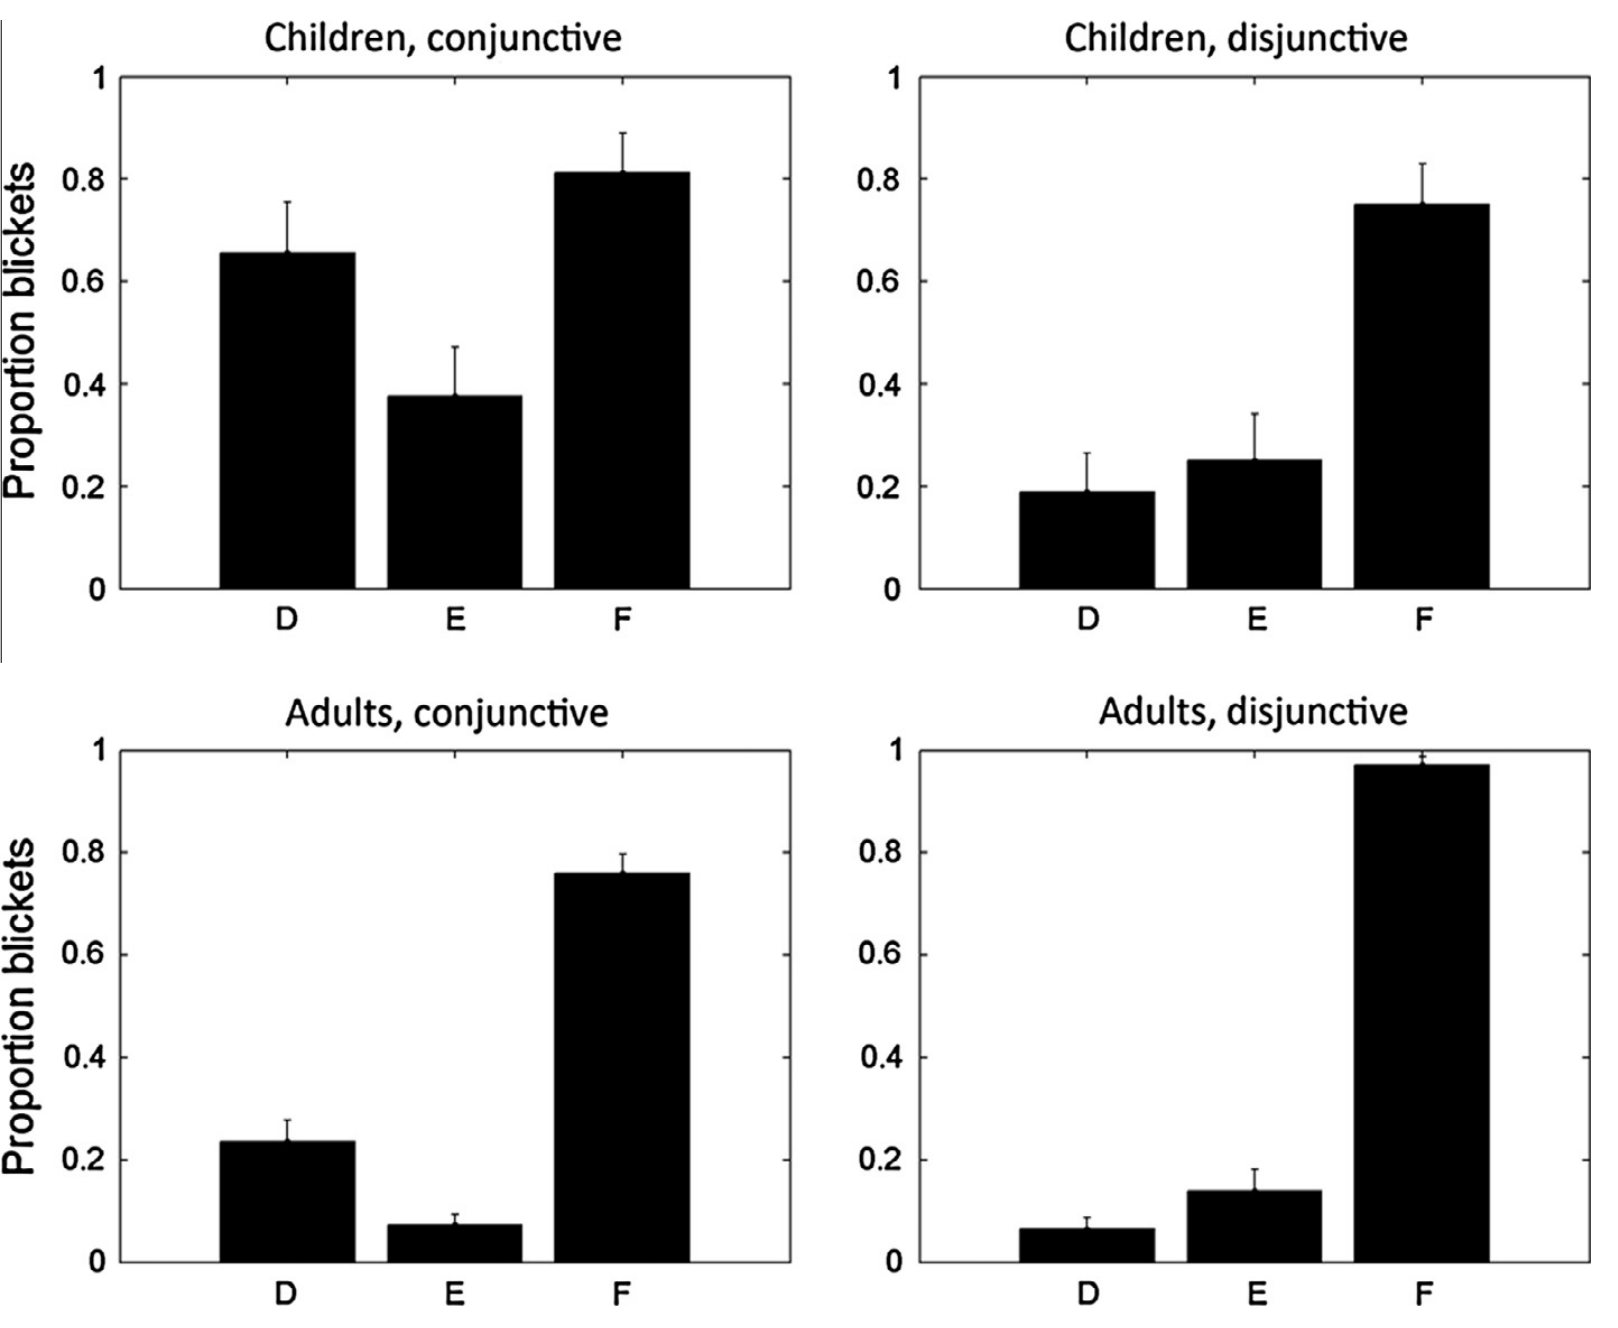
\includegraphics[scale=0.25]{images/experiment1results.png}
    \end{center}
    \end{block}
\end{frame}

\begin{frame}[fragile]
  \frametitle{\shortt: Experimento 1}

    \begin{block}{Resultados}

        \begin{itemize}
        \item Los niños utilizaron los datos de entrenamiento en ambas condiciones.
        \item Niños y adultos se comportaron de la misma forma con la forma disyuntiva.
        \item Los niños aseguran que D y E podrían ser un blicket en la forma conjuntiva.
        \item Los adultos no tomaron en cuenta el entrenamiento conjuntivo y sólo aceptaron a F como respuesta.
        \end{itemize}
        
        Esto afirma las hipótesis sobre el experimento.
    \end{block}

\end{frame}

\begin{frame}[fragile]
  \frametitle{\shortt: Experimento 1}

    \begin{block}{Interpretación}
    \begin{itemize}
    \item Los niños pueden ser más propensos a indicar que cualquier objeto es un blicket.
    \item Los niños se confundieron con el entrenamiento conjuntivo y respondieron sobre D y E, respondiendo randómicamente.
    \item Falta de información sobre E pudo implicar que no sea elegido como blicket.
    \item No se testean los conocimientos causales si no el uso de términos como "blicket", por lo que se utiliza la idea de "blicketness" para incentivar se considere la posibilidad conjuntiva.
    \end{itemize}
    \end{block}
    \begin{block}{Problemas}
    Si la última explicación es correcta, niños y adultos deberían comportarse de igual forma cuando se les pide activar la máquina.
    Sin embargo si infieren diferentes formas causales en las dos condiciones, deberían usar sólo un bloque para activarla en la forma disyuntiva, pero deberían intentar con combinaciones en la forma conjuntiva.
    De igual forma los adultos usarían sólo un bloque para activar la máquina en ambas condiciones.
    
    Para eliminar hipótesis alternativas, se realizó un segundo experimento.
    \end{block}



\end{frame}

\begin{frame}[fragile]
  \frametitle{\shortt: Metodología}

Experimento 2, diferencias:

\begin{itemize}
\item Se pregunta que objetos usarían para activar la máquina.
\item Se modificaron los eventos de prueba para que todos los objetos tengan la misma probabilidad de activar la máquina. (D - D - D - E - DF+ - DEF+ - DF+ ).
\item Se agrega un nuevo objeto G, al que se lo llama \textit{novel object} que no participa en el experimento.
\item Se agrega un nuevo baseline en donde se omite el entrenamiento de los individuos.
\item Se simplifica el procedimiento dando sólo una prueba en vez de dos, pero se repite el entrenamiento dos veces.
\end{itemize}


\end{frame}

\begin{frame}[fragile]
  \frametitle{\shortt: Metodología}

Experimento 2, predicciones:

\begin{itemize}
\item Los niños en el caso disyuntivo deberían devir que F es blicket y los demás no. Indicar que con un solo objeto se activa la máquina.
\item Los niños en el caso conjuntivo deben decir que F y D son blickets y dudar sobre E. Para activar la máquina precisan un conjunto de objetos.
\item 
\end{itemize}


\end{frame}

\section{Conclusión}
\begin{frame}[fragile]
  \frametitle{\shortt: Conclusión}
    
    \begin{exampleblock}{Conclusiones}
    \begin{itemize}
       \item Se observó la habilidad de los niños para adquirir conocimiento abstracto sobre formas de relaciones causales y mostrar que en algunos casos ellos aprenden mejor que los adultos.
       \item En este paper se muestra como niños de 4 a 5 años aprenden estos principios  y los utilizan para la toma de decisiones. En algunos casos los niños aprenden estos principios abstractos más fácilmente que los adultos.

    \end{itemize}
    \end{exampleblock}
\end{frame}


\plain{}{Preguntas}

\end{document}
